\documentclass[tikz,convert={outfile=\jobname.svg}]{standalone}\usepackage{pgfplots}

\pgfplotsset{
	compat = 1.5.1,
	axis equal
	%width = 1.2\linewidth,
	%height = 1.2\linewidth
}

\begin{document}

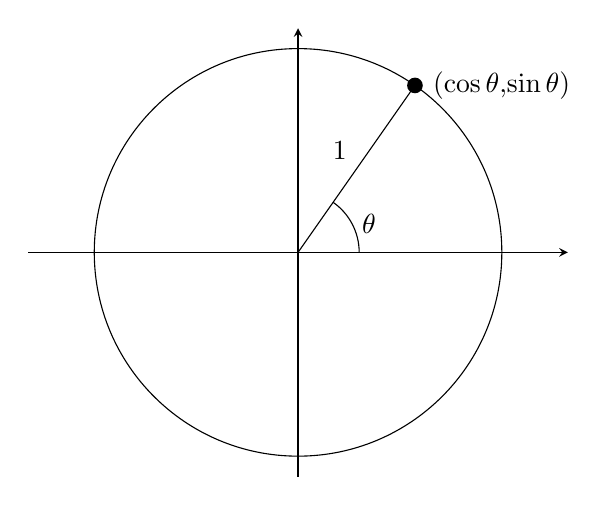
\begin{tikzpicture}
	\begin{axis}[
	axis lines = middle,
	ticks = none,
	xmin = -1.1, xmax = 1.1,
	ymin = -1.1, ymax = 1.1
	]
		\draw (axis cs: 0, 0) circle [radius=1];
		\draw (axis cs: 0, 0) -- (axis cs: 0.5736, 0.8192) node [midway, above left] {$1$};
		\draw (axis cs:0.3,0) arc[start angle=0, end angle=55, radius={transformdirectionx(0.3)}] node [midway, right] {$\theta$};
		\node[label={0:{($\cos\theta$,$\sin\theta$)}},circle,fill,inner sep=2pt] at (axis cs:0.5736,0.8192) {};
	\end{axis}
\end{tikzpicture}

\end{document}